\documentclass[]{article}
\usepackage{lmodern}
\usepackage{amssymb,amsmath}
\usepackage{ifxetex,ifluatex}
\usepackage{fixltx2e} % provides \textsubscript
\ifnum 0\ifxetex 1\fi\ifluatex 1\fi=0 % if pdftex
  \usepackage[T1]{fontenc}
  \usepackage[utf8]{inputenc}
\else % if luatex or xelatex
  \ifxetex
    \usepackage{mathspec}
  \else
    \usepackage{fontspec}
  \fi
  \defaultfontfeatures{Ligatures=TeX,Scale=MatchLowercase}
\fi
% use upquote if available, for straight quotes in verbatim environments
\IfFileExists{upquote.sty}{\usepackage{upquote}}{}
% use microtype if available
\IfFileExists{microtype.sty}{%
\usepackage{microtype}
\UseMicrotypeSet[protrusion]{basicmath} % disable protrusion for tt fonts
}{}
\usepackage[margin=2.54cm]{geometry}
\usepackage{hyperref}
\hypersetup{unicode=true,
            pdftitle={Assignment 8: Time Series Analysis},
            pdfauthor={Sarah Ko},
            pdfborder={0 0 0},
            breaklinks=true}
\urlstyle{same}  % don't use monospace font for urls
\usepackage{color}
\usepackage{fancyvrb}
\newcommand{\VerbBar}{|}
\newcommand{\VERB}{\Verb[commandchars=\\\{\}]}
\DefineVerbatimEnvironment{Highlighting}{Verbatim}{commandchars=\\\{\}}
% Add ',fontsize=\small' for more characters per line
\usepackage{framed}
\definecolor{shadecolor}{RGB}{248,248,248}
\newenvironment{Shaded}{\begin{snugshade}}{\end{snugshade}}
\newcommand{\KeywordTok}[1]{\textcolor[rgb]{0.13,0.29,0.53}{\textbf{#1}}}
\newcommand{\DataTypeTok}[1]{\textcolor[rgb]{0.13,0.29,0.53}{#1}}
\newcommand{\DecValTok}[1]{\textcolor[rgb]{0.00,0.00,0.81}{#1}}
\newcommand{\BaseNTok}[1]{\textcolor[rgb]{0.00,0.00,0.81}{#1}}
\newcommand{\FloatTok}[1]{\textcolor[rgb]{0.00,0.00,0.81}{#1}}
\newcommand{\ConstantTok}[1]{\textcolor[rgb]{0.00,0.00,0.00}{#1}}
\newcommand{\CharTok}[1]{\textcolor[rgb]{0.31,0.60,0.02}{#1}}
\newcommand{\SpecialCharTok}[1]{\textcolor[rgb]{0.00,0.00,0.00}{#1}}
\newcommand{\StringTok}[1]{\textcolor[rgb]{0.31,0.60,0.02}{#1}}
\newcommand{\VerbatimStringTok}[1]{\textcolor[rgb]{0.31,0.60,0.02}{#1}}
\newcommand{\SpecialStringTok}[1]{\textcolor[rgb]{0.31,0.60,0.02}{#1}}
\newcommand{\ImportTok}[1]{#1}
\newcommand{\CommentTok}[1]{\textcolor[rgb]{0.56,0.35,0.01}{\textit{#1}}}
\newcommand{\DocumentationTok}[1]{\textcolor[rgb]{0.56,0.35,0.01}{\textbf{\textit{#1}}}}
\newcommand{\AnnotationTok}[1]{\textcolor[rgb]{0.56,0.35,0.01}{\textbf{\textit{#1}}}}
\newcommand{\CommentVarTok}[1]{\textcolor[rgb]{0.56,0.35,0.01}{\textbf{\textit{#1}}}}
\newcommand{\OtherTok}[1]{\textcolor[rgb]{0.56,0.35,0.01}{#1}}
\newcommand{\FunctionTok}[1]{\textcolor[rgb]{0.00,0.00,0.00}{#1}}
\newcommand{\VariableTok}[1]{\textcolor[rgb]{0.00,0.00,0.00}{#1}}
\newcommand{\ControlFlowTok}[1]{\textcolor[rgb]{0.13,0.29,0.53}{\textbf{#1}}}
\newcommand{\OperatorTok}[1]{\textcolor[rgb]{0.81,0.36,0.00}{\textbf{#1}}}
\newcommand{\BuiltInTok}[1]{#1}
\newcommand{\ExtensionTok}[1]{#1}
\newcommand{\PreprocessorTok}[1]{\textcolor[rgb]{0.56,0.35,0.01}{\textit{#1}}}
\newcommand{\AttributeTok}[1]{\textcolor[rgb]{0.77,0.63,0.00}{#1}}
\newcommand{\RegionMarkerTok}[1]{#1}
\newcommand{\InformationTok}[1]{\textcolor[rgb]{0.56,0.35,0.01}{\textbf{\textit{#1}}}}
\newcommand{\WarningTok}[1]{\textcolor[rgb]{0.56,0.35,0.01}{\textbf{\textit{#1}}}}
\newcommand{\AlertTok}[1]{\textcolor[rgb]{0.94,0.16,0.16}{#1}}
\newcommand{\ErrorTok}[1]{\textcolor[rgb]{0.64,0.00,0.00}{\textbf{#1}}}
\newcommand{\NormalTok}[1]{#1}
\usepackage{graphicx,grffile}
\makeatletter
\def\maxwidth{\ifdim\Gin@nat@width>\linewidth\linewidth\else\Gin@nat@width\fi}
\def\maxheight{\ifdim\Gin@nat@height>\textheight\textheight\else\Gin@nat@height\fi}
\makeatother
% Scale images if necessary, so that they will not overflow the page
% margins by default, and it is still possible to overwrite the defaults
% using explicit options in \includegraphics[width, height, ...]{}
\setkeys{Gin}{width=\maxwidth,height=\maxheight,keepaspectratio}
\IfFileExists{parskip.sty}{%
\usepackage{parskip}
}{% else
\setlength{\parindent}{0pt}
\setlength{\parskip}{6pt plus 2pt minus 1pt}
}
\setlength{\emergencystretch}{3em}  % prevent overfull lines
\providecommand{\tightlist}{%
  \setlength{\itemsep}{0pt}\setlength{\parskip}{0pt}}
\setcounter{secnumdepth}{0}
% Redefines (sub)paragraphs to behave more like sections
\ifx\paragraph\undefined\else
\let\oldparagraph\paragraph
\renewcommand{\paragraph}[1]{\oldparagraph{#1}\mbox{}}
\fi
\ifx\subparagraph\undefined\else
\let\oldsubparagraph\subparagraph
\renewcommand{\subparagraph}[1]{\oldsubparagraph{#1}\mbox{}}
\fi

%%% Use protect on footnotes to avoid problems with footnotes in titles
\let\rmarkdownfootnote\footnote%
\def\footnote{\protect\rmarkdownfootnote}

%%% Change title format to be more compact
\usepackage{titling}

% Create subtitle command for use in maketitle
\providecommand{\subtitle}[1]{
  \posttitle{
    \begin{center}\large#1\end{center}
    }
}

\setlength{\droptitle}{-2em}

  \title{Assignment 8: Time Series Analysis}
    \pretitle{\vspace{\droptitle}\centering\huge}
  \posttitle{\par}
    \author{Sarah Ko}
    \preauthor{\centering\large\emph}
  \postauthor{\par}
    \date{}
    \predate{}\postdate{}
  

\begin{document}
\maketitle

\subsection{OVERVIEW}\label{overview}

This exercise accompanies the lessons in Environmental Data Analytics
(ENV872L) on time series analysis.

\subsection{Directions}\label{directions}

\begin{enumerate}
\def\labelenumi{\arabic{enumi}.}
\tightlist
\item
  Change ``Student Name'' on line 3 (above) with your name.
\item
  Use the lesson as a guide. It contains code that can be modified to
  complete the assignment.
\item
  Work through the steps, \textbf{creating code and output} that fulfill
  each instruction.
\item
  Be sure to \textbf{answer the questions} in this assignment document.
  Space for your answers is provided in this document and is indicated
  by the ``\textgreater{}'' character. If you need a second paragraph be
  sure to start the first line with ``\textgreater{}''. You should
  notice that the answer is highlighted in green by RStudio.
\item
  When you have completed the assignment, \textbf{Knit} the text and
  code into a single PDF file. You will need to have the correct
  software installed to do this (see Software Installation Guide) Press
  the \texttt{Knit} button in the RStudio scripting panel. This will
  save the PDF output in your Assignments folder.
\item
  After Knitting, please submit the completed exercise (PDF file) to the
  dropbox in Sakai. Please add your last name into the file name (e.g.,
  ``Salk\_A08\_TimeSeries.pdf'') prior to submission.
\end{enumerate}

The completed exercise is due on Tuesday, 19 March, 2019 before class
begins.

\subsection{Brainstorm a project
topic}\label{brainstorm-a-project-topic}

\begin{enumerate}
\def\labelenumi{\arabic{enumi}.}
\tightlist
\item
  Spend 15 minutes brainstorming ideas for a project topic, and look for
  a dataset if you are choosing your own rather than using a class
  dataset. Remember your topic choices are due by the end of March, and
  you should post your choice ASAP to the forum on Sakai.
\end{enumerate}

Question: Did you do this?

\begin{quote}
ANSWER: Yes I did! I chose my own dataset and have described my project
goals in the Sakai forum.
\end{quote}

\subsection{Set up your session}\label{set-up-your-session}

\begin{enumerate}
\def\labelenumi{\arabic{enumi}.}
\setcounter{enumi}{1}
\tightlist
\item
  Set up your session. Upload the EPA air quality raw dataset for PM2.5
  in 2018, and the processed NTL-LTER dataset for nutrients in Peter and
  Paul lakes. Build a ggplot theme and set it as your default theme.
  Make sure date variables are set to a date format.
\end{enumerate}

\begin{Shaded}
\begin{Highlighting}[]
\CommentTok{# load packages}
\KeywordTok{library}\NormalTok{(dplyr)}
\end{Highlighting}
\end{Shaded}

\begin{verbatim}
## Warning: package 'dplyr' was built under R version 3.5.2
\end{verbatim}

\begin{verbatim}
## 
## Attaching package: 'dplyr'
\end{verbatim}

\begin{verbatim}
## The following objects are masked from 'package:stats':
## 
##     filter, lag
\end{verbatim}

\begin{verbatim}
## The following objects are masked from 'package:base':
## 
##     intersect, setdiff, setequal, union
\end{verbatim}

\begin{Shaded}
\begin{Highlighting}[]
\KeywordTok{library}\NormalTok{(tidyverse)}
\end{Highlighting}
\end{Shaded}

\begin{verbatim}
## Warning: package 'tidyverse' was built under R version 3.5.2
\end{verbatim}

\begin{verbatim}
## -- Attaching packages --------------------------------------------------------------- tidyverse 1.2.1 --
\end{verbatim}

\begin{verbatim}
## v ggplot2 3.1.0     v readr   1.3.1
## v tibble  2.1.1     v purrr   0.3.2
## v tidyr   0.8.3     v stringr 1.4.0
## v ggplot2 3.1.0     v forcats 0.4.0
\end{verbatim}

\begin{verbatim}
## Warning: package 'ggplot2' was built under R version 3.5.2
\end{verbatim}

\begin{verbatim}
## Warning: package 'tibble' was built under R version 3.5.3
\end{verbatim}

\begin{verbatim}
## Warning: package 'tidyr' was built under R version 3.5.2
\end{verbatim}

\begin{verbatim}
## Warning: package 'readr' was built under R version 3.5.2
\end{verbatim}

\begin{verbatim}
## Warning: package 'purrr' was built under R version 3.5.3
\end{verbatim}

\begin{verbatim}
## Warning: package 'stringr' was built under R version 3.5.2
\end{verbatim}

\begin{verbatim}
## Warning: package 'forcats' was built under R version 3.5.2
\end{verbatim}

\begin{verbatim}
## -- Conflicts ------------------------------------------------------------------ tidyverse_conflicts() --
## x dplyr::filter() masks stats::filter()
## x dplyr::lag()    masks stats::lag()
\end{verbatim}

\begin{Shaded}
\begin{Highlighting}[]
\KeywordTok{library}\NormalTok{(tidyr)}
\KeywordTok{library}\NormalTok{(ggpubr)}
\end{Highlighting}
\end{Shaded}

\begin{verbatim}
## Warning: package 'ggpubr' was built under R version 3.5.2
\end{verbatim}

\begin{verbatim}
## Loading required package: magrittr
\end{verbatim}

\begin{verbatim}
## 
## Attaching package: 'magrittr'
\end{verbatim}

\begin{verbatim}
## The following object is masked from 'package:purrr':
## 
##     set_names
\end{verbatim}

\begin{verbatim}
## The following object is masked from 'package:tidyr':
## 
##     extract
\end{verbatim}

\begin{Shaded}
\begin{Highlighting}[]
\KeywordTok{library}\NormalTok{(lubridate)}
\end{Highlighting}
\end{Shaded}

\begin{verbatim}
## Warning: package 'lubridate' was built under R version 3.5.2
\end{verbatim}

\begin{verbatim}
## 
## Attaching package: 'lubridate'
\end{verbatim}

\begin{verbatim}
## The following object is masked from 'package:base':
## 
##     date
\end{verbatim}

\begin{Shaded}
\begin{Highlighting}[]
\KeywordTok{library}\NormalTok{(nlme)}
\end{Highlighting}
\end{Shaded}

\begin{verbatim}
## 
## Attaching package: 'nlme'
\end{verbatim}

\begin{verbatim}
## The following object is masked from 'package:dplyr':
## 
##     collapse
\end{verbatim}

\begin{Shaded}
\begin{Highlighting}[]
\KeywordTok{library}\NormalTok{(multcompView)}
\end{Highlighting}
\end{Shaded}

\begin{verbatim}
## Warning: package 'multcompView' was built under R version 3.5.2
\end{verbatim}

\begin{Shaded}
\begin{Highlighting}[]
\KeywordTok{library}\NormalTok{(lme4)}
\end{Highlighting}
\end{Shaded}

\begin{verbatim}
## Warning: package 'lme4' was built under R version 3.5.3
\end{verbatim}

\begin{verbatim}
## Loading required package: Matrix
\end{verbatim}

\begin{verbatim}
## 
## Attaching package: 'Matrix'
\end{verbatim}

\begin{verbatim}
## The following object is masked from 'package:tidyr':
## 
##     expand
\end{verbatim}

\begin{verbatim}
## 
## Attaching package: 'lme4'
\end{verbatim}

\begin{verbatim}
## The following object is masked from 'package:nlme':
## 
##     lmList
\end{verbatim}

\begin{Shaded}
\begin{Highlighting}[]
\KeywordTok{library}\NormalTok{(trend)}
\end{Highlighting}
\end{Shaded}

\begin{verbatim}
## Warning: package 'trend' was built under R version 3.5.2
\end{verbatim}

\begin{Shaded}
\begin{Highlighting}[]
\CommentTok{# get working directory}
\KeywordTok{getwd}\NormalTok{()}
\end{Highlighting}
\end{Shaded}

\begin{verbatim}
## [1] "C:/Users/Sarah/Documents/Duke/Year 2/Spring 2019/Data Analytics/Environmental_Data_Analytics"
\end{verbatim}

\begin{Shaded}
\begin{Highlighting}[]
\CommentTok{# set wd to filepath of Environmental_Data_Analytics to use relative filepath}
\CommentTok{# load EPA air quality raw dataset for PM2.5 in 2018}
\NormalTok{Air_PM25_}\DecValTok{2018}\NormalTok{ <-}\StringTok{ }\KeywordTok{read.csv}\NormalTok{(}\StringTok{"./Data/Raw/EPAair_PM25_NC2018_raw.csv"}\NormalTok{)}

\CommentTok{# load NTL-LTER for nutrients in Peter and Paul Lakes}
\NormalTok{NTL_Nutrients_PeterPaul <-}
\StringTok{  }\KeywordTok{read.csv}\NormalTok{(}\StringTok{"./Data/Processed/NTL-LTER_Lake_Nutrients_PeterPaulGathered_Processed.csv"}\NormalTok{)}

\CommentTok{# build ggplot theme, set as default theme}
\NormalTok{SKotheme <-}\StringTok{ }\KeywordTok{theme_gray}\NormalTok{(}\DataTypeTok{base_size =} \DecValTok{15}\NormalTok{) }\OperatorTok{+}
\KeywordTok{theme}\NormalTok{(}\DataTypeTok{axis.text =} \KeywordTok{element_text}\NormalTok{(}\DataTypeTok{color =} \StringTok{"black"}\NormalTok{),}
\DataTypeTok{legend.position =} \StringTok{"right"}\NormalTok{,}
\DataTypeTok{plot.title =} \KeywordTok{element_text}\NormalTok{(}\DataTypeTok{hjust =} \FloatTok{0.5}\NormalTok{))}
\KeywordTok{theme_set}\NormalTok{(SKotheme)}

\CommentTok{# check date variables}
\KeywordTok{class}\NormalTok{(Air_PM25_}\DecValTok{2018}\OperatorTok{$}\NormalTok{Date)}
\end{Highlighting}
\end{Shaded}

\begin{verbatim}
## [1] "factor"
\end{verbatim}

\begin{Shaded}
\begin{Highlighting}[]
\KeywordTok{class}\NormalTok{(NTL_Nutrients_PeterPaul}\OperatorTok{$}\NormalTok{sampledate)}
\end{Highlighting}
\end{Shaded}

\begin{verbatim}
## [1] "factor"
\end{verbatim}

\begin{Shaded}
\begin{Highlighting}[]
\CommentTok{# change date variables to date must define original format of data}
\NormalTok{Air_PM25_}\DecValTok{2018}\OperatorTok{$}\NormalTok{Date <-}\StringTok{ }\KeywordTok{as.Date}\NormalTok{(Air_PM25_}\DecValTok{2018}\OperatorTok{$}\NormalTok{Date, }\DataTypeTok{format =} \StringTok{"%m/%d/%y"}\NormalTok{)}
\NormalTok{NTL_Nutrients_PeterPaul}\OperatorTok{$}\NormalTok{sampledate <-}\StringTok{ }\KeywordTok{as.Date}\NormalTok{(NTL_Nutrients_PeterPaul}\OperatorTok{$}\NormalTok{sampledate, }\DataTypeTok{format =} \StringTok{"%Y-%m-%d"}\NormalTok{)}

\CommentTok{# confirm date variables}
\KeywordTok{class}\NormalTok{(Air_PM25_}\DecValTok{2018}\OperatorTok{$}\NormalTok{Date)}
\end{Highlighting}
\end{Shaded}

\begin{verbatim}
## [1] "Date"
\end{verbatim}

\begin{Shaded}
\begin{Highlighting}[]
\KeywordTok{class}\NormalTok{(NTL_Nutrients_PeterPaul}\OperatorTok{$}\NormalTok{sampledate)}
\end{Highlighting}
\end{Shaded}

\begin{verbatim}
## [1] "Date"
\end{verbatim}

\subsection{Run a hierarchical (mixed-effects)
model}\label{run-a-hierarchical-mixed-effects-model}

Research question: Do PM2.5 concentrations have a significant trend in
2018?

\begin{enumerate}
\def\labelenumi{\arabic{enumi}.}
\setcounter{enumi}{2}
\tightlist
\item
  Run a repeated measures ANOVA, with PM2.5 concentrations as the
  response, Date as a fixed effect, and Site.Name as a random effect.
  This will allow us to extrapolate PM2.5 concentrations across North
  Carolina.
\end{enumerate}

3a. Illustrate PM2.5 concentrations by date. Do not split aesthetics by
site.

\begin{Shaded}
\begin{Highlighting}[]
\CommentTok{# 3) run repeated measures ANOVA}
\NormalTok{PM25_repeat_measures <-}\StringTok{ }\KeywordTok{lme}\NormalTok{(}\DataTypeTok{data =}\NormalTok{ Air_PM25_}\DecValTok{2018}\NormalTok{,}
\NormalTok{                     Daily.Mean.PM2.}\FloatTok{5.}\NormalTok{Concentration }\OperatorTok{~}\StringTok{ }\NormalTok{Date, }
                     \DataTypeTok{random =} \OperatorTok{~}\DecValTok{1}\OperatorTok{|}\NormalTok{Site.Name)}
\NormalTok{PM25_repeat_measures}
\end{Highlighting}
\end{Shaded}

\begin{verbatim}
## Linear mixed-effects model fit by REML
##   Data: Air_PM25_2018 
##   Log-restricted-likelihood: -20297.38
##   Fixed: Daily.Mean.PM2.5.Concentration ~ Date 
## (Intercept)        Date 
## 20.14183588 -0.00074241 
## 
## Random effects:
##  Formula: ~1 | Site.Name
##         (Intercept) Residual
## StdDev:    1.841425 3.457061
## 
## Number of Observations: 7611
## Number of Groups: 24
\end{verbatim}

\begin{Shaded}
\begin{Highlighting}[]
\CommentTok{# 3a) graph PM2.5 by date}
\NormalTok{PM25_date <-}\StringTok{ }\KeywordTok{ggplot}\NormalTok{(}\DataTypeTok{data =}\NormalTok{ Air_PM25_}\DecValTok{2018}\NormalTok{, }\KeywordTok{aes}\NormalTok{(}\DataTypeTok{x =}\NormalTok{ Date, }\DataTypeTok{y =}\NormalTok{ Daily.Mean.PM2.}\FloatTok{5.}\NormalTok{Concentration)) }\OperatorTok{+}\StringTok{   }
\StringTok{  }\KeywordTok{geom_point}\NormalTok{(}\DataTypeTok{alpha=}\FloatTok{0.5}\NormalTok{, }\DataTypeTok{stroke=}\DecValTok{0}\NormalTok{) }\OperatorTok{+}\StringTok{ }
\StringTok{  }\KeywordTok{ggtitle}\NormalTok{(}\StringTok{"PM 2.5 Concentration over Time"}\NormalTok{) }\OperatorTok{+}\StringTok{ }\CommentTok{# add main title}
\StringTok{  }\KeywordTok{xlab}\NormalTok{(}\StringTok{"Date"}\NormalTok{) }\OperatorTok{+}
\StringTok{  }\KeywordTok{ylab}\NormalTok{(}\StringTok{"Daily Mean PM 2.5 Concentration (\textbackslash{}U003BCg/m^3)"}\NormalTok{)}
\KeywordTok{print}\NormalTok{(PM25_date)}
\end{Highlighting}
\end{Shaded}

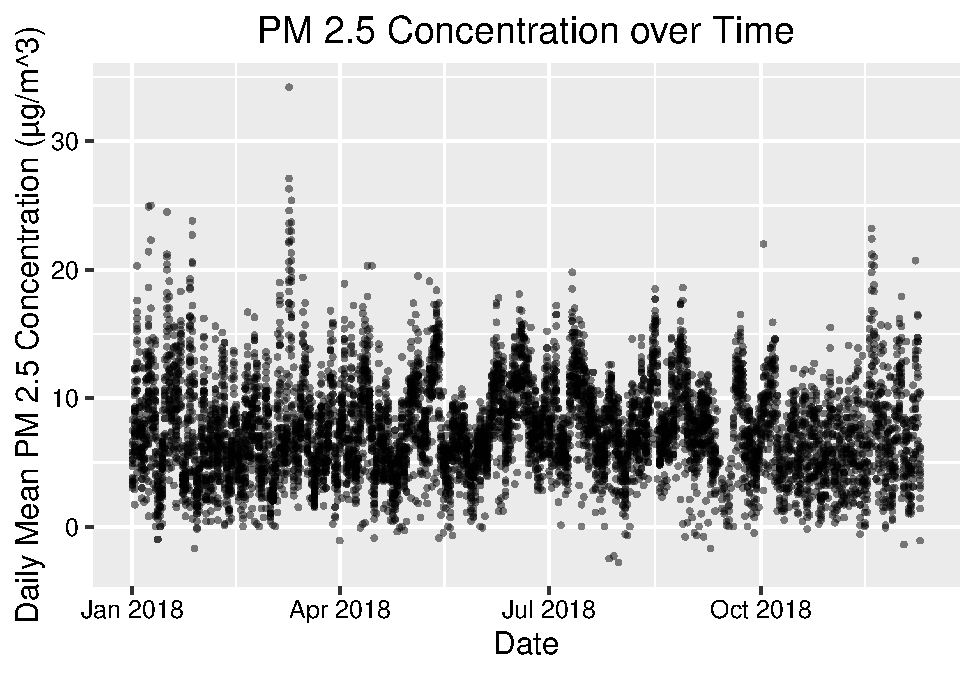
\includegraphics{A08_TimeSeries_files/figure-latex/unnamed-chunk-2-1.pdf}

3b. Insert the following line of code into your R chunk. This will
eliminate duplicate measurements on single dates for each site. PM2.5 =
PM2.5{[}order(PM2.5{[},`Date'{]},-PM2.5{[},`Site.ID'{]}),{]} PM2.5 =
PM2.5{[}!duplicated(PM2.5\$Date),{]}

3c. Determine the temporal autocorrelation in your model.

3d. Run a mixed effects model.

\begin{Shaded}
\begin{Highlighting}[]
\CommentTok{# 3b) eliminate duplicate measurements on single dates for each site}
\NormalTok{PM2.}\DecValTok{5}\NormalTok{ <-}\StringTok{ }\NormalTok{Air_PM25_}\DecValTok{2018}

\NormalTok{PM2.}\DecValTok{5}\NormalTok{ =}\StringTok{ }\NormalTok{PM2.}\DecValTok{5}\NormalTok{[}\KeywordTok{order}\NormalTok{(PM2.}\DecValTok{5}\NormalTok{[,}\StringTok{'Date'}\NormalTok{],}\OperatorTok{-}\NormalTok{PM2.}\DecValTok{5}\NormalTok{[,}\StringTok{'Site.ID'}\NormalTok{]),]}
\NormalTok{PM2.}\DecValTok{5}\NormalTok{ =}\StringTok{ }\NormalTok{PM2.}\DecValTok{5}\NormalTok{[}\OperatorTok{!}\KeywordTok{duplicated}\NormalTok{(PM2.}\DecValTok{5}\OperatorTok{$}\NormalTok{Date),]}

\CommentTok{# 3c) determine temporal autocorrelation}
\KeywordTok{ACF}\NormalTok{(PM25_repeat_measures)}
\end{Highlighting}
\end{Shaded}

\begin{verbatim}
##    lag          ACF
## 1    0  1.000000000
## 2    1  0.473017989
## 3    2  0.143093030
## 4    3  0.060500838
## 5    4  0.061574447
## 6    5  0.087756109
## 7    6  0.061116723
## 8    7  0.007595491
## 9    8  0.025491472
## 10   9  0.057872193
## 11  10  0.095911195
## 12  11  0.086519308
## 13  12  0.041507759
## 14  13  0.041091743
## 15  14  0.008663124
## 16  15 -0.012810524
## 17  16 -0.016388970
## 18  17 -0.023436707
## 19  18  0.020967717
## 20  19  0.032373855
## 21  20 -0.046770645
## 22  21 -0.086974675
## 23  22 -0.045009633
## 24  23  0.014507171
## 25  24  0.046279402
## 26  25  0.021031653
## 27  26 -0.017185250
## 28  27  0.008158717
\end{verbatim}

\begin{Shaded}
\begin{Highlighting}[]
\CommentTok{# take the 2nd value (the innermost group level) to define the degree of autocorrelation = 0.473017989}

\CommentTok{# 3d) run mixed effects model}
\NormalTok{PM25_mixed_effects <-}\StringTok{ }\KeywordTok{lme}\NormalTok{(}\DataTypeTok{data =}\NormalTok{ PM2.}\DecValTok{5}\NormalTok{,}
\NormalTok{                     Daily.Mean.PM2.}\FloatTok{5.}\NormalTok{Concentration }\OperatorTok{~}\StringTok{ }\NormalTok{Date, }
                     \DataTypeTok{random =} \OperatorTok{~}\DecValTok{1}\OperatorTok{|}\NormalTok{Site.Name, }\CommentTok{#specify autocorrelation structure of order 1}
                     \DataTypeTok{method =} \StringTok{"REML"}\NormalTok{) }\CommentTok{#define method as restricted maximum likelihood}
\KeywordTok{summary}\NormalTok{(PM25_mixed_effects)}
\end{Highlighting}
\end{Shaded}

\begin{verbatim}
## Linear mixed-effects model fit by REML
##  Data: PM2.5 
##        AIC      BIC    logLik
##   1865.215 1880.543 -928.6076
## 
## Random effects:
##  Formula: ~1 | Site.Name
##         (Intercept) Residual
## StdDev:    1.650184 3.559209
## 
## Fixed effects: Daily.Mean.PM2.5.Concentration ~ Date 
##                Value Std.Error  DF   t-value p-value
## (Intercept) 90.46502  34.57133 339  2.616764  0.0093
## Date        -0.00473   0.00195 339 -2.425102  0.0158
##  Correlation: 
##      (Intr)
## Date -0.999
## 
## Standardized Within-Group Residuals:
##         Min          Q1         Med          Q3         Max 
## -2.38072443 -0.63365107 -0.09616694  0.61426094  3.42056220 
## 
## Number of Observations: 343
## Number of Groups: 3
\end{verbatim}

Is there a significant increasing or decreasing trend in PM2.5
concentrations in 2018?

\begin{quote}
ANSWER: There is a significant decreasing trend in PM2.5 concentrations
in 2018. The model equation is: concentration of PM2.5 (ug/m3) =
90.46502 - 0.00473*date. The p values corresponding to the intercept and
the date variable are significant, with p = 0.0093 and p = 0.0158
respectively.
\end{quote}

3e. Run a fixed effects model with Date as the only explanatory
variable. Then test whether the mixed effects model is a better fit than
the fixed effect model.

\begin{Shaded}
\begin{Highlighting}[]
\CommentTok{# 3e) run fixed effect model with Date as the only explanatory variable}
\NormalTok{PM25_date_only <-}\StringTok{ }\KeywordTok{gls}\NormalTok{(}\DataTypeTok{data =}\NormalTok{ PM2.}\DecValTok{5}\NormalTok{,}
\NormalTok{                     Daily.Mean.PM2.}\FloatTok{5.}\NormalTok{Concentration }\OperatorTok{~}\StringTok{ }\NormalTok{Date,}
                     \DataTypeTok{method =} \StringTok{"REML"}\NormalTok{) }\CommentTok{# no random effect, no autocorrelation structure}
\KeywordTok{summary}\NormalTok{(PM25_date_only)}
\end{Highlighting}
\end{Shaded}

\begin{verbatim}
## Generalized least squares fit by REML
##   Model: Daily.Mean.PM2.5.Concentration ~ Date 
##   Data: PM2.5 
##        AIC      BIC    logLik
##   1865.202 1876.698 -929.6011
## 
## Coefficients:
##                Value Std.Error   t-value p-value
## (Intercept) 98.57796  34.60285  2.848840  0.0047
## Date        -0.00513   0.00195 -2.624999  0.0091
## 
##  Correlation: 
##      (Intr)
## Date -1    
## 
## Standardized residuals:
##        Min         Q1        Med         Q3        Max 
## -2.3531000 -0.6348100 -0.1153454  0.6383004  3.4063068 
## 
## Residual standard error: 3.584321 
## Degrees of freedom: 343 total; 341 residual
\end{verbatim}

\begin{Shaded}
\begin{Highlighting}[]
\KeywordTok{anova}\NormalTok{(PM25_mixed_effects, PM25_date_only)}
\end{Highlighting}
\end{Shaded}

\begin{verbatim}
##                    Model df      AIC      BIC    logLik   Test  L.Ratio
## PM25_mixed_effects     1  4 1865.215 1880.543 -928.6076                
## PM25_date_only         2  3 1865.202 1876.698 -929.6011 1 vs 2 1.986919
##                    p-value
## PM25_mixed_effects        
## PM25_date_only      0.1587
\end{verbatim}

Which model is better?

\begin{quote}
ANSWER: The mixed effects model has an AIC value of 1865.215. The fixed
effect model with only date as the explanatory variable has a slightly
lower AIC value of 1865.202, indicating it to be the better model.
However, the p value is 0.1587, which indicates that the models do not
have a significantly different fit.
\end{quote}

\subsection{Run a Mann-Kendall test}\label{run-a-mann-kendall-test}

Research question: Is there a trend in total N surface concentrations in
Peter and Paul lakes?

\begin{enumerate}
\def\labelenumi{\arabic{enumi}.}
\setcounter{enumi}{3}
\tightlist
\item
  Duplicate the Mann-Kendall test we ran for total P in class, this time
  with total N for both lakes. Make sure to run a test for changepoints
  in the datasets (and run a second one if a second change point is
  likely).
\end{enumerate}

\begin{Shaded}
\begin{Highlighting}[]
\CommentTok{# Wrangle dataset}
\NormalTok{NTL_PeterPaul_TotalN <-}\StringTok{ }
\StringTok{  }\NormalTok{NTL_Nutrients_PeterPaul }\OperatorTok
\StringTok{  }\KeywordTok{select}\NormalTok{(}\OperatorTok{-}\NormalTok{daynum, }\OperatorTok{-}\NormalTok{year4) }\OperatorTok
\StringTok{  }\KeywordTok{filter}\NormalTok{(nutrient }\OperatorTok{==}\StringTok{ "tn_ug"}\NormalTok{) }\OperatorTok
\StringTok{  }\KeywordTok{filter}\NormalTok{(depth }\OperatorTok{==}\StringTok{ }\DecValTok{0}\NormalTok{)}

\CommentTok{# initial visualization of the data}
\NormalTok{Total_N_plot <-}\StringTok{ }\KeywordTok{ggplot}\NormalTok{(NTL_PeterPaul_TotalN, }\KeywordTok{aes}\NormalTok{(}\DataTypeTok{x =}\NormalTok{ sampledate, }\DataTypeTok{y =}\NormalTok{ concentration, }
                                                 \DataTypeTok{color =}\NormalTok{ lakename)) }\OperatorTok{+}\StringTok{ }
\StringTok{  }\KeywordTok{geom_point}\NormalTok{() }\OperatorTok{+}\StringTok{ }
\StringTok{  }\KeywordTok{scale_color_manual}\NormalTok{(}\DataTypeTok{values =} \KeywordTok{c}\NormalTok{(}\StringTok{"#7fcdbb"}\NormalTok{, }\StringTok{"#253494"}\NormalTok{)) }\OperatorTok{+}\StringTok{ }
\StringTok{  }\KeywordTok{ggtitle}\NormalTok{(}\StringTok{"Total N in Peter and Paul Lakes"}\NormalTok{) }\OperatorTok{+}\StringTok{ }\CommentTok{# add main title}
\StringTok{  }\KeywordTok{xlab}\NormalTok{(}\StringTok{"Date"}\NormalTok{) }\OperatorTok{+}
\StringTok{  }\KeywordTok{ylab}\NormalTok{(}\StringTok{"Total N (\textbackslash{}U003BCg/L)"}\NormalTok{)}
\KeywordTok{print}\NormalTok{(Total_N_plot)}
\end{Highlighting}
\end{Shaded}

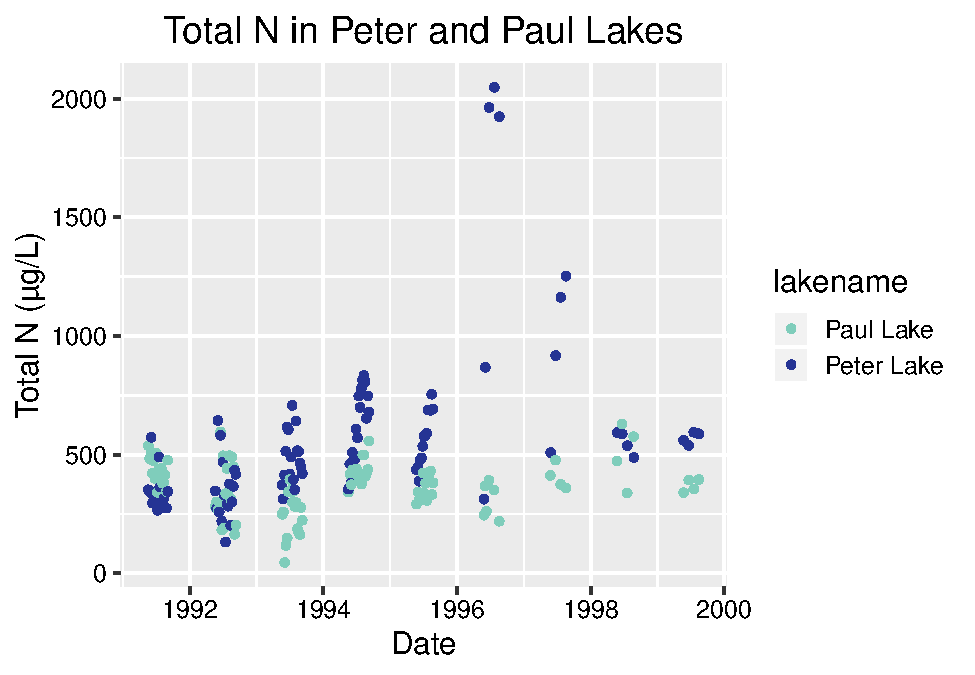
\includegraphics{A08_TimeSeries_files/figure-latex/unnamed-chunk-5-1.pdf}

\begin{Shaded}
\begin{Highlighting}[]
\NormalTok{Peter.N.surface <-}\StringTok{ }\KeywordTok{filter}\NormalTok{(NTL_PeterPaul_TotalN, lakename }\OperatorTok{==}\StringTok{ "Peter Lake"}\NormalTok{)}
\KeywordTok{dim}\NormalTok{(Peter.N.surface) }\CommentTok{# length = 98}
\end{Highlighting}
\end{Shaded}

\begin{verbatim}
## [1] 98  5
\end{verbatim}

\begin{Shaded}
\begin{Highlighting}[]
\NormalTok{Paul.N.surface <-}\StringTok{ }\KeywordTok{filter}\NormalTok{(NTL_PeterPaul_TotalN, lakename }\OperatorTok{==}\StringTok{ "Paul Lake"}\NormalTok{)}
\KeywordTok{dim}\NormalTok{(Paul.N.surface) }\CommentTok{# length = 99}
\end{Highlighting}
\end{Shaded}

\begin{verbatim}
## [1] 99  5
\end{verbatim}

\begin{Shaded}
\begin{Highlighting}[]
\CommentTok{# PETER LAKE}
\CommentTok{# Run a Mann-Kendall test}
\KeywordTok{mk.test}\NormalTok{(Peter.N.surface}\OperatorTok{$}\NormalTok{concentration)}
\end{Highlighting}
\end{Shaded}

\begin{verbatim}
## 
##  Mann-Kendall trend test
## 
## data:  Peter.N.surface$concentration
## z = 7.2927, n = 98, p-value = 3.039e-13
## alternative hypothesis: true S is not equal to 0
## sample estimates:
##            S         varS          tau 
## 2.377000e+03 1.061503e+05 5.001052e-01
\end{verbatim}

\begin{Shaded}
\begin{Highlighting}[]
\CommentTok{# Test Peter Lake for changepoints}
\KeywordTok{pettitt.test}\NormalTok{(Peter.N.surface}\OperatorTok{$}\NormalTok{concentration) }\CommentTok{# change point at time = 36}
\end{Highlighting}
\end{Shaded}

\begin{verbatim}
## 
##  Pettitt's test for single change-point detection
## 
## data:  Peter.N.surface$concentration
## U* = 1884, p-value = 3.744e-10
## alternative hypothesis: two.sided
## sample estimates:
## probable change point at time K 
##                              36
\end{verbatim}

\begin{Shaded}
\begin{Highlighting}[]
\NormalTok{Peter.N.surface}\OperatorTok{$}\NormalTok{sampledate[}\DecValTok{35}\NormalTok{] }\CommentTok{# 1993-05-26}
\end{Highlighting}
\end{Shaded}

\begin{verbatim}
## [1] "1993-05-26"
\end{verbatim}

\begin{Shaded}
\begin{Highlighting}[]
\NormalTok{Peter.N.surface}\OperatorTok{$}\NormalTok{sampledate[}\DecValTok{36}\NormalTok{] }\CommentTok{# 1993-06-02}
\end{Highlighting}
\end{Shaded}

\begin{verbatim}
## [1] "1993-06-02"
\end{verbatim}

\begin{Shaded}
\begin{Highlighting}[]
\CommentTok{# change point at ~ 1993-05-29}

\CommentTok{# Run separate Mann-Kendall for each change point}
\KeywordTok{mk.test}\NormalTok{(Peter.N.surface}\OperatorTok{$}\NormalTok{concentration[}\DecValTok{1}\OperatorTok{:}\DecValTok{35}\NormalTok{])}
\end{Highlighting}
\end{Shaded}

\begin{verbatim}
## 
##  Mann-Kendall trend test
## 
## data:  Peter.N.surface$concentration[1:35]
## z = -0.22722, n = 35, p-value = 0.8203
## alternative hypothesis: true S is not equal to 0
## sample estimates:
##             S          varS           tau 
##  -17.00000000 4958.33333333   -0.02857143
\end{verbatim}

\begin{Shaded}
\begin{Highlighting}[]
\KeywordTok{mk.test}\NormalTok{(Peter.N.surface}\OperatorTok{$}\NormalTok{concentration[}\DecValTok{36}\OperatorTok{:}\DecValTok{98}\NormalTok{])}
\end{Highlighting}
\end{Shaded}

\begin{verbatim}
## 
##  Mann-Kendall trend test
## 
## data:  Peter.N.surface$concentration[36:98]
## z = 3.1909, n = 63, p-value = 0.001418
## alternative hypothesis: true S is not equal to 0
## sample estimates:
##            S         varS          tau 
## 5.390000e+02 2.842700e+04 2.759857e-01
\end{verbatim}

\begin{Shaded}
\begin{Highlighting}[]
\CommentTok{# check for second change point}
\KeywordTok{pettitt.test}\NormalTok{(Peter.N.surface}\OperatorTok{$}\NormalTok{concentration[}\DecValTok{36}\OperatorTok{:}\DecValTok{98}\NormalTok{]) }\CommentTok{# change point at time = 36+21 = 57}
\end{Highlighting}
\end{Shaded}

\begin{verbatim}
## 
##  Pettitt's test for single change-point detection
## 
## data:  Peter.N.surface$concentration[36:98]
## U* = 560, p-value = 0.001213
## alternative hypothesis: two.sided
## sample estimates:
## probable change point at time K 
##                              21
\end{verbatim}

\begin{Shaded}
\begin{Highlighting}[]
\NormalTok{Peter.N.surface}\OperatorTok{$}\NormalTok{sampledate[}\DecValTok{56}\NormalTok{] }\CommentTok{# 1994-06-22}
\end{Highlighting}
\end{Shaded}

\begin{verbatim}
## [1] "1994-06-22"
\end{verbatim}

\begin{Shaded}
\begin{Highlighting}[]
\NormalTok{Peter.N.surface}\OperatorTok{$}\NormalTok{sampledate[}\DecValTok{57}\NormalTok{] }\CommentTok{# 1994-06-29}
\end{Highlighting}
\end{Shaded}

\begin{verbatim}
## [1] "1994-06-29"
\end{verbatim}

\begin{Shaded}
\begin{Highlighting}[]
\CommentTok{# change point at ~ 1994-06-25}

\CommentTok{# PAUL LAKE}
\CommentTok{# Run a Mann-Kendall test}
\KeywordTok{mk.test}\NormalTok{(Paul.N.surface}\OperatorTok{$}\NormalTok{concentration)}
\end{Highlighting}
\end{Shaded}

\begin{verbatim}
## 
##  Mann-Kendall trend test
## 
## data:  Paul.N.surface$concentration
## z = -0.35068, n = 99, p-value = 0.7258
## alternative hypothesis: true S is not equal to 0
## sample estimates:
##             S          varS           tau 
## -1.170000e+02  1.094170e+05 -2.411874e-02
\end{verbatim}

\begin{Shaded}
\begin{Highlighting}[]
\CommentTok{# Test Paul Lake for changepoints}
\KeywordTok{pettitt.test}\NormalTok{(Paul.N.surface}\OperatorTok{$}\NormalTok{concentration) }\CommentTok{# possible change point at time = 16, }
\end{Highlighting}
\end{Shaded}

\begin{verbatim}
## 
##  Pettitt's test for single change-point detection
## 
## data:  Paul.N.surface$concentration
## U* = 704, p-value = 0.09624
## alternative hypothesis: two.sided
## sample estimates:
## probable change point at time K 
##                              16
\end{verbatim}

\begin{Shaded}
\begin{Highlighting}[]
\CommentTok{#but p value is not significant}
\end{Highlighting}
\end{Shaded}

What are the results of this test?

\begin{quote}
ANSWER: Peter Lake shows a significant change in total N surface
concentrations over time. It is seen to have 2 change points: the first
\textasciitilde{}1993-05-29 (p \textless{} 0.01), and the second
\textasciitilde{}1994-06-25 (p \textless{} 0.01). Paul Lake does not
show any significant change points.
\end{quote}

\begin{enumerate}
\def\labelenumi{\arabic{enumi}.}
\setcounter{enumi}{4}
\tightlist
\item
  Generate a graph that illustrates the TN concentrations over time,
  coloring by lake and adding vertical line(s) representing
  changepoint(s).
\end{enumerate}

\begin{Shaded}
\begin{Highlighting}[]
\CommentTok{# graph with changepoints}
\NormalTok{Total_N_plot_changepoints <-}\StringTok{ }\KeywordTok{ggplot}\NormalTok{(NTL_PeterPaul_TotalN, }\KeywordTok{aes}\NormalTok{(}\DataTypeTok{x =}\NormalTok{ sampledate, }
                                                              \DataTypeTok{y =}\NormalTok{ concentration, }\DataTypeTok{color =}\NormalTok{ lakename)) }\OperatorTok{+}\StringTok{ }
\StringTok{  }\KeywordTok{geom_point}\NormalTok{() }\OperatorTok{+}\StringTok{ }
\StringTok{  }\KeywordTok{scale_color_manual}\NormalTok{(}\DataTypeTok{values =} \KeywordTok{c}\NormalTok{(}\StringTok{"#7fcdbb"}\NormalTok{, }\StringTok{"#253494"}\NormalTok{)) }\OperatorTok{+}\StringTok{ }
\StringTok{  }\KeywordTok{ggtitle}\NormalTok{(}\StringTok{"Total N in Peter and Paul Lakes"}\NormalTok{) }\OperatorTok{+}\StringTok{ }\CommentTok{# add main title}
\StringTok{  }\KeywordTok{xlab}\NormalTok{(}\StringTok{"Date"}\NormalTok{) }\OperatorTok{+}
\StringTok{  }\KeywordTok{ylab}\NormalTok{(}\StringTok{"Total N (\textbackslash{}U003BCg/L)"}\NormalTok{) }\OperatorTok{+}\StringTok{ }
\StringTok{  }\KeywordTok{geom_vline}\NormalTok{(}\DataTypeTok{xintercept =} \KeywordTok{as.Date}\NormalTok{(}\StringTok{"1993-05-29"}\NormalTok{), }\DataTypeTok{linetype=}\DecValTok{2}\NormalTok{, }
                \DataTypeTok{color =} \StringTok{"#253494"}\NormalTok{, }\DataTypeTok{size=}\FloatTok{1.5}\NormalTok{) }\OperatorTok{+}\StringTok{ }
\StringTok{  }\KeywordTok{geom_vline}\NormalTok{(}\DataTypeTok{xintercept =} \KeywordTok{as.Date}\NormalTok{(}\StringTok{"1994-06-25"}\NormalTok{), }\DataTypeTok{linetype=}\DecValTok{2}\NormalTok{, }
                \DataTypeTok{color =} \StringTok{"#253494"}\NormalTok{, }\DataTypeTok{size=}\FloatTok{1.5}\NormalTok{)}
\KeywordTok{print}\NormalTok{(Total_N_plot_changepoints)}
\end{Highlighting}
\end{Shaded}

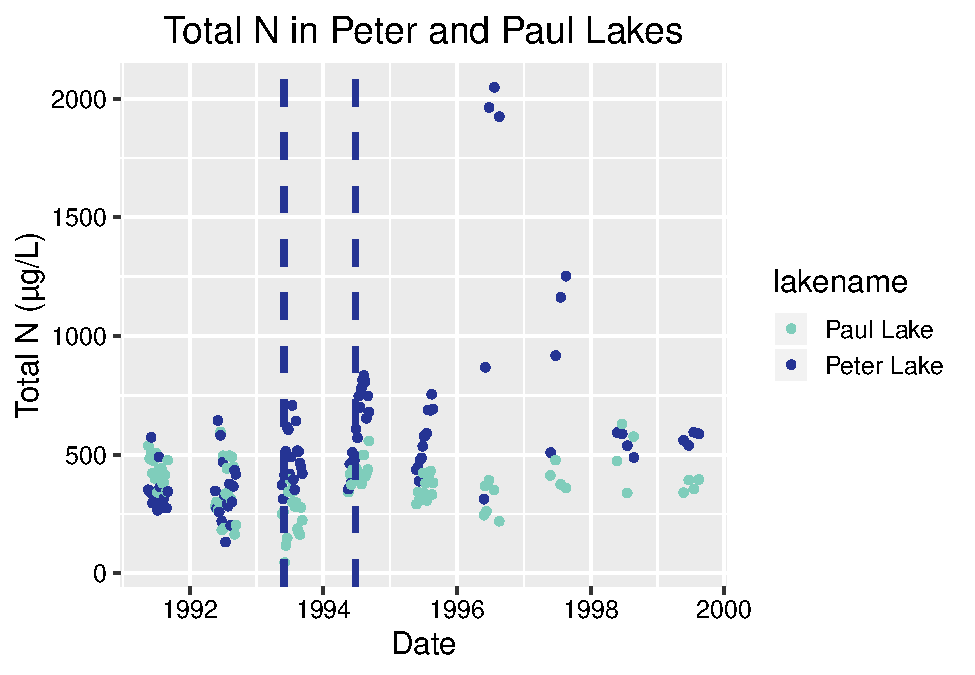
\includegraphics{A08_TimeSeries_files/figure-latex/unnamed-chunk-6-1.pdf}


\end{document}
